\section{Delsystem}

Systemet är indelat i två olika delsystem. Dessa system kommer köras
sekvensiellt, alltså det ena efter det andra. Det första systemet kontrollerar
själva bilkörningen medan det andra systemet kontrollerar displayen. Se
figur~\ref{fig:system_diagram} för ett processchema.

\begin{figure}
  \centering
  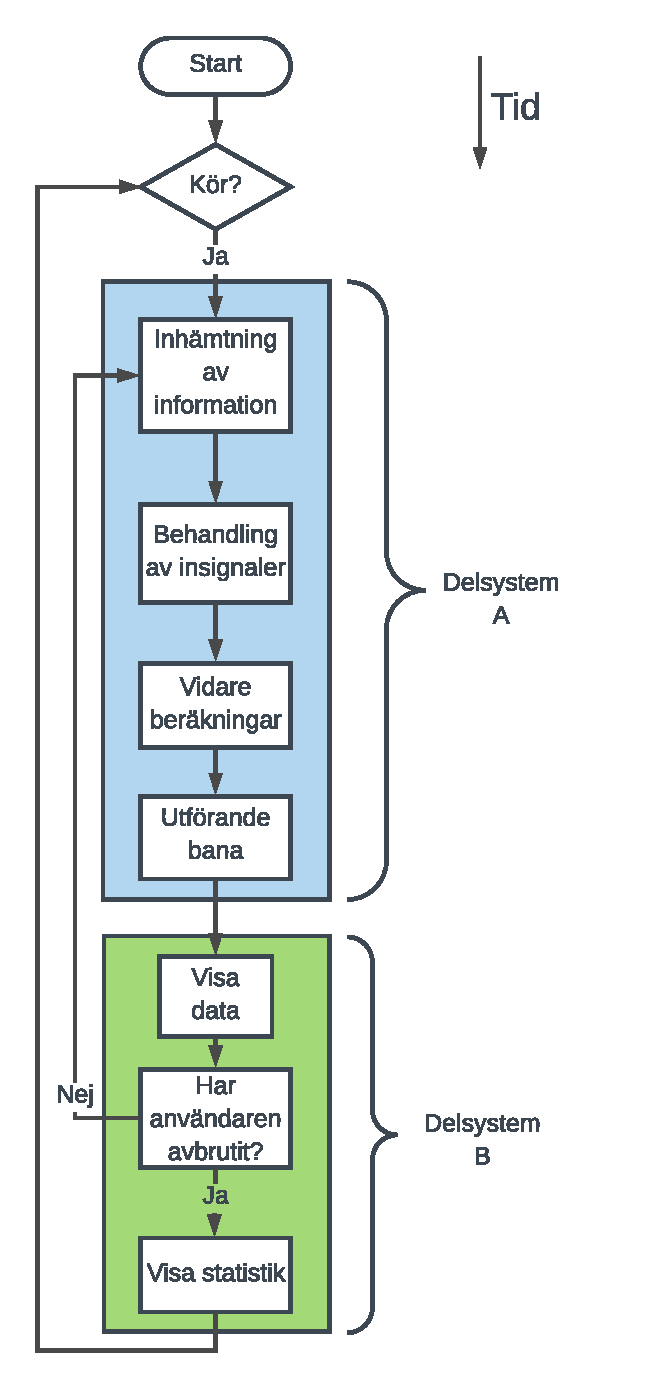
\includegraphics[width=\linewidth,height=0.9\textheight,keepaspectratio]{figures/Processchema.pdf}
  \caption{Processchema över systemets helhet.}%
  \label{fig:system_diagram}
\end{figure}

  \subsection{Delsystem A: Bana}
  
  Delsystem A är indelat i tre övergripande delar. I del A.1 hämtas all
  tillgänglig information in, i del A.2a görs beräkningar utifrån tillgänglig
  data, i del A.2b görs vidare beräkningar (alltså beräkningar som inte baseras
  direkt på den tillgängliga informationen), och i del A.3 utförs de ändringar
  som programmet bedömer är nödvändiga för att klara den valda varvtiden. 

    \subsubsection{Inhämtning av information}

    Information som finns tillgänglig är kraftigt begränsad. I praktiken kommer
    programmet endast fråga om någon av bilarna passerat en givare sedan
    programmet frågade förra gången.

    \subsubsection{Primära beräkningar}

    De primära beräkningarna är de beräkningar som beror direkt på tillgänglig
    information. Eftersom indatan enbart består av bilens position är bilens
    hastighet genom det förra segmentet den enda informationen som direkt beror
    på indata.

    \subsubsection{Sekundära beräkningar}
    
    Den första beräkningen som görs är bilens nuvarande position. Detta görs med
    hjälp av en intern bild av banan och vetskapen om vilken hastighet bilen
    önskas ha. Sedan räknas den position som bäst gör att bilen klarar den satta
    varvtiden ut. För att räkna ut den beaktas enbart den nuvarande tiden och
    (om gemensam målgång är aktiverat) positionen av den andra bilen. Steget
    efter är att räkna ut den mest rimliga optimala situationen som beaktar hur
    lång tid det är kvar på det nuvarande varvet. I början av varvet görs alltså
    inte lika drastiska hastighetsändringar som mot slutet.

    Det sista som händer är när informationen om bilens och banans skick används
    för att räkna ut vilket spänningspådrag som krävs för att få bilen att nå
    den hastighet och position som krävs.

    \subsubsection{Utförande}

    I utförandet skickas det nya spänningspådraget till banorna. 
	

    \subsubsection{Funktioner i delsystem A} \label{sec:system_a_funcs}
    I figur~\ref{fig:flow_diagram}  visas flödet av de funktioner som sker i delsystem A under en cykel.
    Här listas namn på funktionerna och deras funktion:
    \begin{itemize}
	\item old\textunderscore u: old u är lagring av data från bilens spänning. Denna databas kommer lagra information om tidigare cyklar, varv och tidigare lopp. Databasen kommer vara en egen separat funktion så att det blir lätt att referera till databasen.
	\item old\textunderscore v: old v är lagringen av data från bilens hastighet mellan segment, varv, tidigare lopp och detta lagras i databasen som är en egen funktion som vi kommer att referera till. 
	\item old\textunderscore position: Lagring av gammal data för bilens placering. Från denna databas kan andra funktioner få information om var bilen var förra cykeln, var bilen var för ett varv sedan m.m.
      \item indata: Ger data när bilen passerar en givare.
      \item car\textunderscore constant: Programmets sätt att anpassa sig efter olika bilars egenskaper. Justeras vid varje ny indata.
      \item position: Position, programmet räknar ut vart på banan bilen befinner sig genom att hämta senaste positionen old position och sedan addera sträckan bilen har färdats sedan dess senaste värde. Sträckan som bilen har färdats kan räknas ut genom S=V\textasteriskcentered T, där v = old\textunderscore v och (delta)t = tidskillnaden mellan senaste cykel. Om ny indata finns denna cykel så är positionen känd och denna data används i stället för att utgå igrån gammal.
      \item clock: Hur länge bilen har varit i det nuvarande segmentet och varvet.

      \item car\textunderscore position\textunderscore dif: Endast aktiv om gemensam målgång aktiverad. Jämför bilarnas position med varandra. Funktionen utgår ifrån respektive bils placering (från old\textunderscore position) och hastighet (från old\textunderscore v) 
och ger ett värde på placeringsskillnaden för en viss hastighet. Detta kommer
sedan användas för att sätta bilarnas nya hastighet. Värdet blir stort om skillnaden i placering är stor men justeras också efter hastigeten. Dvs om bilarna ligger långt ifrån varandra men åker ganska fort kommer inte värdet bli lika stort som om bilarna legat lika långt ifrån varandra men haft lägre hastighet. Värdet är positivt om bil 1 ligger före bil 2 och negativt om bil 2 ligger före bil 1. På så sätt kan nästa funktion avgöra vilken bil som ligger först.
Värdet används sedan för att beräkna nästa hastighet (new\textunderscore v) som kommer ökas eller minskas för att få bilarna att köra ikapp varandra. 

      \item target: Den varvtid som manuellt har satts innan programet startade.
      \item target dif: Den differensen mellan den önskade tiden och positionen relativt till den faktiska tiden och positionen. Görs genom att subtrahera de önskade värdena med de faktiska värdena.  
      \item agressivness: Justerar hur stora ändringar som görs på new\textunderscore v, vid start av ett nytt varv finns det mycket tid kvar att justera. Följden av detta är att new \textunderscore v kan ändras lite i taget istället för att göra stora förändringar. Agressivness räknas ut via; clock,  vilken tid på varvet bilen befinner sig, Target \textunderscore dif,  hur långt ifrån måltiden befinner sig bilen och om gemensam målgång är aktiv tar agresivness även hänsyn till car\textunderscore position \textunderscore dif,  hur långt är avståndet mellan de två bilarna. 
      \item u\textunderscore constant\textunderscore map: Är en kartläggning över banan och de spänningsnivåer som behöver sättas så att spänningen blir jämn. Detta eftersom att spänningstillförseln beter sig olika för olika delar av banan. Kartläggningen kommer bygga på det register med inlagrad data som tagits fram genom tester.
      \item target\textunderscore dif: Bilens position relativt till var den borde vara vid den nuvarande tiden.
      \item track\textunderscore u\textunderscore constant: Detta ät det förbestämda spänningsvärdet för ett visst subsegment på banan. Värdet tas fram manuellt genom prövning och lagras i u \textunderscore constant \textunderscore map. Ur position tar track \textunderscore u \textunderscore constant fram rätt spänningsvärde. 
      \item speed\textunderscore map: En ``karta'' över hur fort man kan köra i olika delar av banan.n.
      \item speed\textunderscore constant: Den förbestämda hastigheten för nuvarande subsegment. Hastigheten tas fram manuellt genom prövning och lagras i speed \textunderscore map. Ur position tar speed \textunderscore constant fram rätt hastighet. 

% new_v     
\item new\textunderscore v: Beräknar den hastighet som bilen ska få nästa cykel. Funktionen tar förra cykelns hastighet (old\textunderscore v) 
och lägger till eller tar bort lite beroende på hur långt ifrån målet som bilarna ligger (target\textunderscore dif) och om gemensam
målgång aktiverad hur långt ifrån varandra bilarna är (car\textunderscore position\textunderscore dif). Funktionen beror 
också på agressivness, högre agressivness ger större skillnad mellan new\textunderscore v och old\textunderscore v medan ett lågt värde gör så att v 
inte kommer ändras särskillt mycket.
new\textunderscore v används sedan för att sätta
new\textunderscore u. Högre new\textunderscore v ger högre new\textunderscore u och lägre new\textunderscore v ger lägre\textunderscore u. 
      \item new\textunderscore u: Beräknar den spänning som ska appliceras beroende på vilken hastighet new \textunderscore v anger. Ett högre new \textunderscore v innebär ett högre new\textunderscore u. De andra parametrarna som påverkar new\textunderscore u är car\textunderscore constant och track\textunderscore u\textunderscore constant, desto högre dessa värden dessa antar desto högre värde antar också new\textunderscore u. New\textunderscore u är programmets sista output, dess värde 0 till 127 är den spänning som appliceras på bilen. Värdet lagras också direkt till loggen old\textunderscore u. 

    \end{itemize}

    \begin{figure}
      \centering
      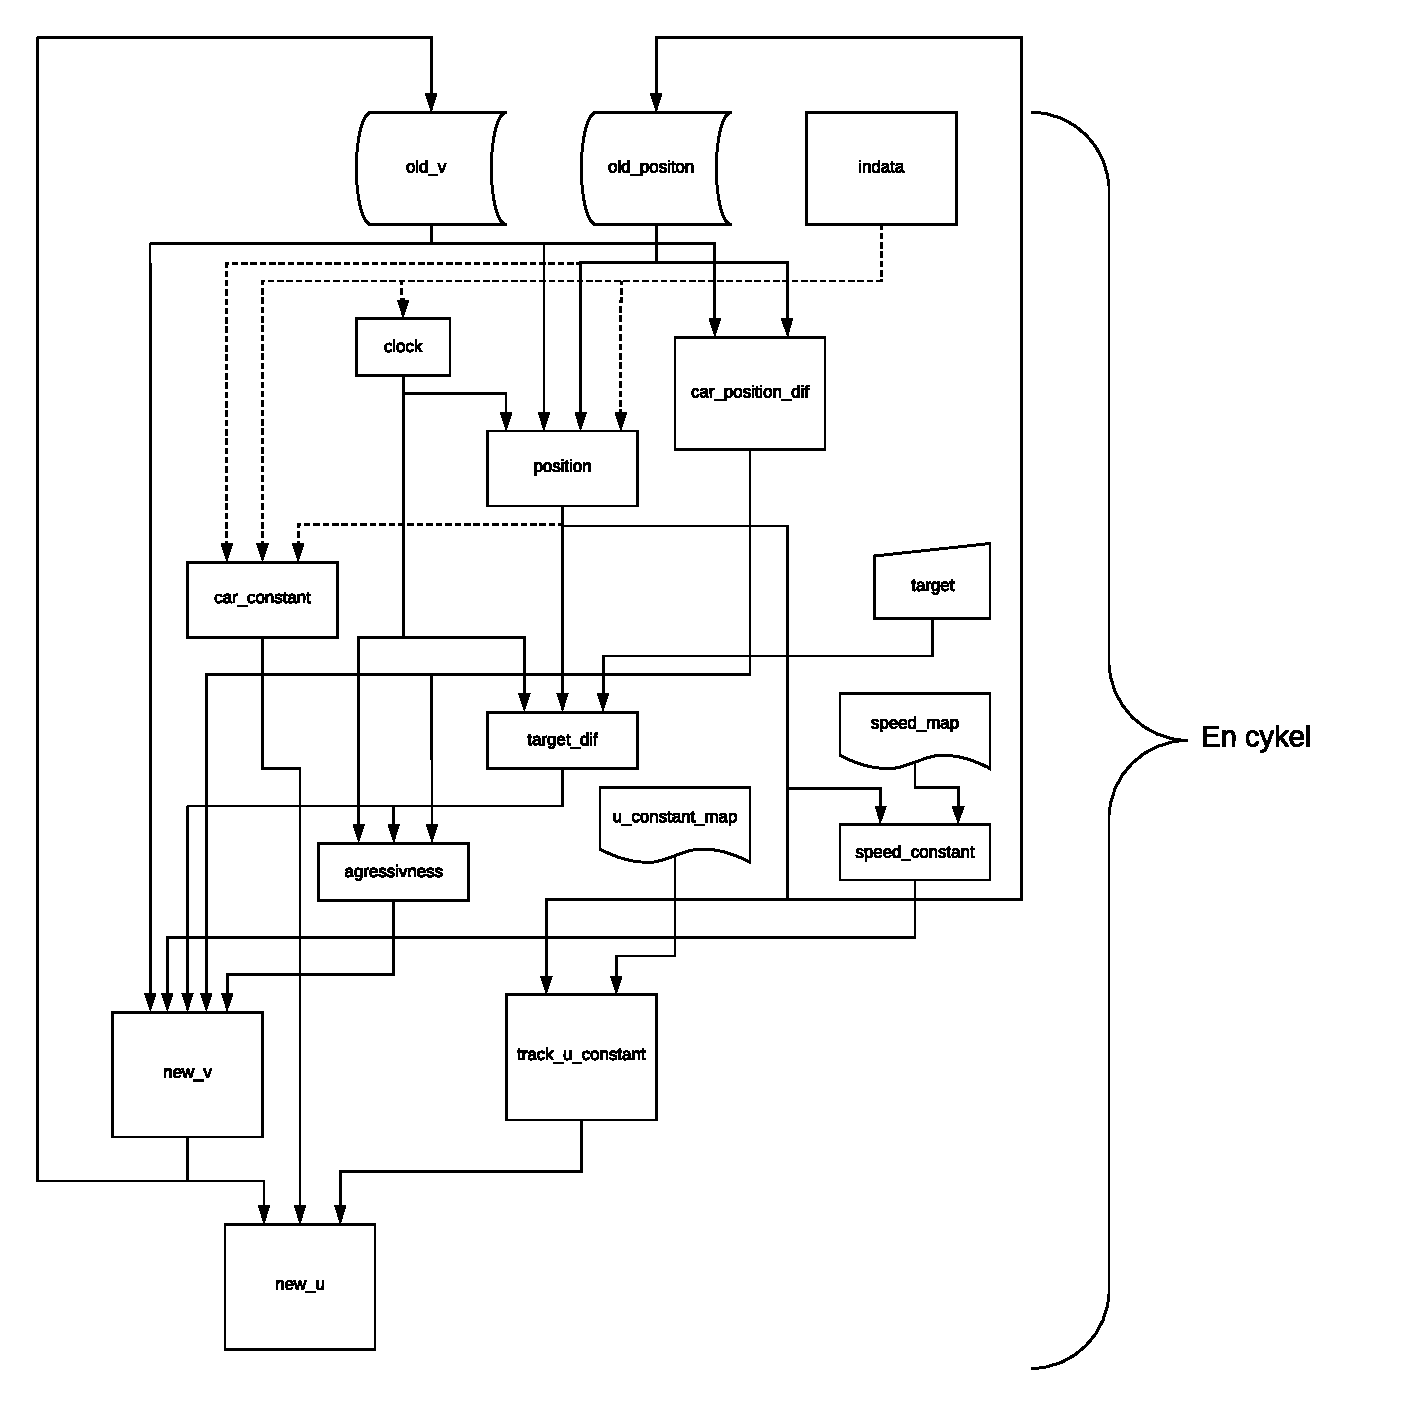
\includegraphics[width=\linewidth]{figures/flow.pdf}
      \caption{Funktionsflödet i delsystem A.}%
      \label{fig:flow_diagram}
    \end{figure}

  \subsection{Delsystem B: Display}

  Displayen ter sig enklare än delsystem A. Under körning ska, om ett nytt varv
  påbörjats, den senaste varvtiden och varvnumret skickas till displayen. Om
  stopp-knappen har tryckts ned ska systemet hoppa till resultat-skärmen och om
  inte så ska det fortsätta.

